\subsection{Stochastic Gradient Descent}

We start with a random weight matrix $W$ and random biases $b$ and $b^{'}$. We take a given input $x$, and feed it forward through the network and compute the error between the target output $t$ and the actual output $z$. Often we use the squared loss error $E(t,z) = \frac{1}{2}\norm{t-z}_2^2$ to determine the difference between the two. In the case of an autoencoder, the target output is the same as the input. If the error is not satisfactory, we can adjust the weight matrix and that biases in order to attempt to learn a better representation of the data. A common method of updating the weight and biases is via backpropogation \cite{hecht1989theory}; when applied to training inputs one at a time, it is also known as stochastic gradient descent (SGD). We will first consider the update for the weights and biases from the last hidden layer to the output layer with a squared loss error function and derive the updates. We use as an example a simple three layer neural network (input, one hidden and output layer). Some notation is given in Table \ref{tab:notation}.

\begin{table}[h]
\normalsize
\begin{tabular}{l|l}
Symbol     & Meaning                                                          \\ \hline
$E$          & Error as computed at the output layer                            \\
$x_j$       & Node $j$ in the input layer                                      \\
$y_j$       & Node $j$ in the hidden layer                                     \\
$z_j$       & Node $j$ in the output layer                                     \\
$n_j$       & $\sum_{i=1}^n W_{ij}x_i + b_j$                                   \\
$t_j$       & Target output at node $j$                                   \\
$W_{ij}^H$ & Weight $i,j$ from input to hidden layer \\
$W_{ij}^O$ & Weight $i,j$ from hidden to output layer \\
$s(x_j)$    & $1/(1+e^{-x_j})$                                                 \\
$b_j^{\{H,O\}}$    & Biases for hidden and output layer                                                \\
\end{tabular}
\caption{Table giving notation for the derivation of updates.}
\label{tab:notation}
\end{table}

The derivative of the output error $E$ with respect to an output matrix weight $W_{ij}^O$ is as follows.

\begin{equation}
\begin{split}
\frac{\partial E}{\partial W^O_{ij}} &= \frac{\partial E}{\partial z_j}\frac{\partial z_j}{\partial W^O_{ij}} \\
																	 &=(z_j - t_j)\frac{\partial s(n_j)}{\partial x_j}\frac{\partial x_j}{\partial W^O_{ij}} \\
																	 &=(z_j-t_j)s(n_j)(1-s(n_j))x_i \\
																	 &=(z_j-t_j)z_j(1-z_j)x_i \\
\end{split}
\label{}
\end{equation}
Now that we have the gradient for the error associated to a single training example, we can compute the updates.
\begin{equation}
\begin{split}
\delta^O_j &= (z_j-t_j)z_j(1-z_j) \\
W^O_{ij} &\leftarrow W^O_{ij} - \eta \delta^O_j x_i \\
b^O_j &\leftarrow b^O_j - \eta\delta^O_j
\end{split}
\end{equation}

The computation of the gradient for the weight matrix between hidden layers is similarly easy to compute.
\begin{equation}
\begin{split}
\frac{\partial E}{\partial W^H_{ij}} &= \frac{\partial E}{\partial y_j}\frac{\partial y_j}{\partial W^H_{ij}} \\
&=\left(\sum_{k=1}^m \frac{\partial E}{\partial z_k}\frac{\partial z_k}{\partial n_k}\frac{\partial n_k}{\partial y_j} \right)\frac{\partial y_j}{\partial n_j}\frac{\partial n_j}{\partial W_{ij}^H}\\
																	 &=\left(\sum_{k=1}^m (z_k - t_k)(1-z_k)z_kW_{jk}^O \right)y_j(1-y_j)x_i
\end{split}
\label{}
\end{equation}
And then using the computed gradient we can define the updates to be used for the hidden layers
\begin{equation}
\begin{split}
\delta^H_j &= \left(\sum_{k=1}^m (z_k - t_k)(1-z_k)z_kW_{jk}^O \right)y_j(1-y_j) \\
W^H_{ij} &\leftarrow W^H_{ij} - \eta\delta^H_jx_i \\
b^H_j &\leftarrow b^H_j - \eta\delta^H_j
\end{split}
\end{equation}

In general, for a neural network we may have different output error functions and these will result in different update rules. We will also give the updates
for the cross-entropy error function with softmax activation in the final layer.
The cross entropy error function is given by $E(x,t) = -\sum_{i=1}^n \left(t_i\ln z_i + (1-t_i)\ln(1-z_i)\right)$
and the softmax function is given by $\sigma(x_j) = e^{x_j} /(\sum_k e^{x_k})$. Following the same procedure as above
for computing the gradient and the updates, we find that for hidden/output layer

\begin{equation}
\begin{split}
\frac{\partial E}{\partial W^O_{ij}} &= (z_j - t_j)y_i \\
\delta^O_j &= (z_j-t_j) \\
W^O_{ij} &\leftarrow W^O_{ij} - \eta \delta^O_j x_i \\
b^O_j &\leftarrow b^O_j - \eta\delta^O_j.
\end{split}
\end{equation}

Note also that we find that the updates for the hidden layer is the same as in the squared error loss function with sigmoid activation. A general overview of the backpropagation algorithm is given by by Algorithm~\ref{alg:backprop}.

The algorithm and derivations for the autoencoder are a slight variation on the above derivations for a more general neural network. In particular, the weight matrix of the output layer (decoding stage) is the transpose of the weight matrix of the hidden layer (encoding stage). Thus $z=s(W^{O}(W^{H}x + b) + b^{'})$, $(W^H)^T = W^O$, and $W^H_{ij} = W^O_{ji}$. 

Once we have trained a single autoencoder layer, we can stack another autoencoder layer on top of the first one for further training. This second autoencoder takes the output of the hidden layer (encoding stage) of the first autoencoder as input and attempts the minimize the input's reconstruction cost.

\begin{algorithm}[h]
\caption{Backpropogation}
\label{alg:backprop}
\begin{algorithmic}
\STATE Initialize the weights and biases randomly
\FOR{iter $=1,2,3...$}
	\FORALL{Examples $x$ in training set (randomize)}
		\STATE $z\gets$ Feedforward $x$
		\STATE Compute output layer $\delta_j^O$
		\STATE ${W_{ij} \leftarrow W_{ij} - \eta \delta^O_j x_i}$
		\STATE $b_j \leftarrow b_j - \eta\delta^O_j$
		\FORALL{Layers in reverse order}
			\STATE Compute hidden layer delta $\delta_k^H$
			\STATE ${W^H_{ij} \leftarrow W^H_{ij} - \eta\delta^H_jx_i}$
			\STATE $b_j \leftarrow b_j - \eta\delta^H_j$
		\ENDFOR
	\ENDFOR
\ENDFOR
\end{algorithmic}
\end{algorithm}

After using backpropogation (or a genetic algorithm) to train each of the autoencoder layers, we can then attach an output layer to the autoencoder to be used for classification. At this
point we use supervised learning to train the output layer and \textit{fine-tune} the autoencoder layers to produce a classifier based on the autoencoder. When pretraining the autoencoder
we train one layer at a time using backpropogation, but during the fine-tuning step we train the entire network via backpropogation, one layer at a time per training image. 


\subsection{Performance}
We note that the steps of backpropagation can only be done in sequence; thus we can only parallelize the operations done within each step. The three major operations which benefit from parallelization are computing the matrix-vector products $W^{H}x$ and $W^{O}y$, computing $\delta^O_j$ and $\delta^H_j$, and updating the entries of the weight matrices with the gradient. For performance reasons we dont store $W^O$ separately; instead we access $W^H$ with transposed indexes when decoding, calculating $\delta^O_j$, and applying the gradient update.

The most expensive parts of the backpropogation algorithm are computing the forward activations of the network and updating the weight matrices for the network. Computing the forward propogation requires performing a matrix-vector multiplication at each layer of the network. The size of that matrix depends on the input and output sizes of that layer. Thus if we have a network with $N$ layers and the sizes of each of those layers is $n_i$, then We have $N$ matrix-vector multiplications of size $n_{i-1} \times n_i$. Updating the weights also has complexity based on the size of the matrix since it requires updating all the entries of the matrix at each iteration.

To improve the performance of these two expensive steps, we parallelized them first using OpenMP and then later parallelized the matrix-vector products using OpenBLAS. Parallelization of these two steps is fairly straight forward and we give some results on scaling below. 


\begin{figure}[h]
\centering
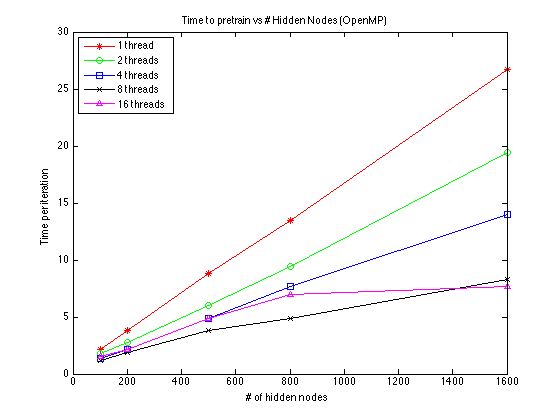
\includegraphics[width=1.0\linewidth]{performanceomp.png}
\caption{Time per iteration versus the number of threads and hidden nodes. We use our own parallel implementation using OpenMP and we use 5000 training images.}
\label{fig:performanceomp}
\end{figure}


\begin{figure}[h]
\centering
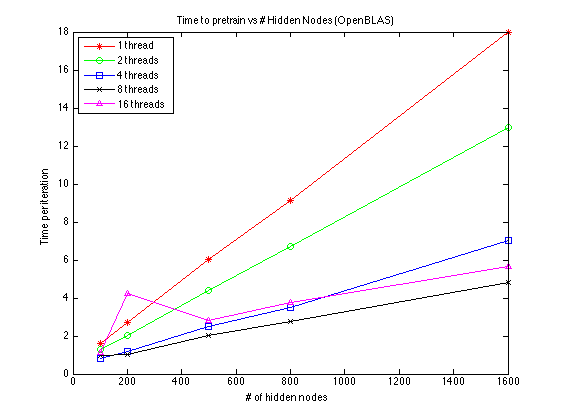
\includegraphics[width=1.0\linewidth]{performanceblas.png}
\caption{Time per iteration versus the number of threads and hidden nodes. We parallelize with OpenBLAS and we use 5000 training images.}
\label{fig:performanceblas}
\end{figure}



\begin{figure}[h]
\centering
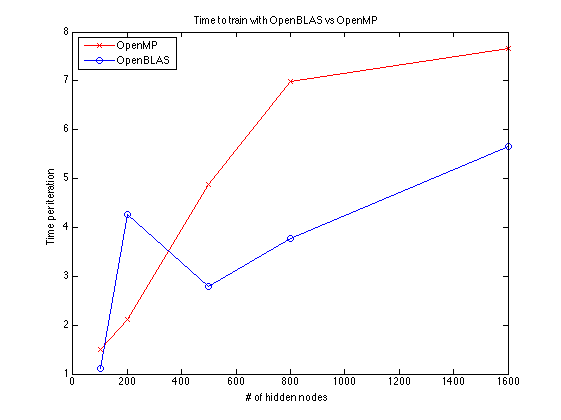
\includegraphics[width=1.0\linewidth]{ompvsblas.png}
\caption{Time per iteration versus parallelization technique and hidden nodes. We use 16 threads here.}
\label{fig:ompvsblas}
\end{figure}

In  Fig.~\ref{fig:performanceomp} we give the performance of training the autoencoder using SGD for different numbers of hidden nodes and different numbers of threads using our own parallel implementation.
In  Fig.~\ref{fig:performanceblas} we give the performance of training the autoencoder using SGD for different numbers of hidden nodes and different numbers of threads using OpenBLAS for parallelization of the matrix-vector multiplies and
matrix-transpose-vector multiplies. The weight updates are not able to be done in OpenBLAS, and so we continue to do that using OpenMP.
We consider the relative performance of these two methods in Fig.~\ref{fig:ompvsblas}.

We note that the Fig.~\ref{fig:performanceomp} and Fig.~\ref{fig:performanceblas} show similar scaling, though in most cases the OpenBLAS version outperforms our own implementation. However, for small numbers of nodes, OpenBLAS does not perform well with many threads.

\subsection{Genetic Algorithm}

A genetic algorithm (GA) is a biologically inspired black-box optimization algorithm is capable of optimizing arbitrary non-convex, non-differential objective functions. The GA works by iteratively improving upon a population of candidate solution vectors (also know as individuals) via genetic operations such as selection, mutation, and crossover. The goal is to maximize the fitness of each individual, which is determined by evaluating the individual with some objective function. In the case of autoencoders, the objective function is the reconstruction loss function defined earlier, the individual is a real valued vector that represents the weights $W$ and biases $b_j^{\{H,O\}}$, and the fitness of an individual is simply $1/E(t,z)$. Algorithm~\ref{alg:genetic} shows the pseudocode of a simple conventional genetic algorithm, which we will refer to as CGA. 

\begin{algorithm}[h]
\caption{Genetic Algorithm}
\label{alg:genetic}
\begin{algorithmic}
\STATE Initialize $N$ individuals randomly
\FOR{iter $=1,2,3...$}
	\STATE Evaluate each individual with objective function and assign fitness
	\STATE Scale fitness of all individuals, typically with a \textbf{power scaling}
	\STATE Select existing individuals via \textbf{roulette selection}
	\FOR{Every two individuals $a$ and $b$ selected}
		\STATE Create copies $a'$ and $b'$
		\STATE Perform \textbf{uniform mutation} on $a'$ and $b'$ with mutation rate $mr$ and mutation amount $ma$
		\STATE Perform \textbf{uniform crossover} using $a'$ and $b'$ with crossover rate $cr$
	\ENDFOR
	\STATE Replace worst $\alpha$ individuals in population with newly created individuals
\ENDFOR
\end{algorithmic}
\end{algorithm}

We will explain step by step what each bold term in the pseudocode means and how it affects individuals in the population:

\begin{itemize}
  \item Power Scaling: All individuals in the population are ranked in ascending order according to their fitness. Each individual is assigned a scaled fitness is is equal to $R^{\gamma}$ where R is the position of the individual within the ranking and $\gamma$ is a parameter to be tuned. Higher values for $\gamma$ will create a scaled fitness distribution that favor individuals with higher actual fitness. Thus $\gamma$ will affect the selection of individuals later and determine how elitist the selection of individuals will be (in other words, how likely will an individual of higher fitness will be selected).
  \item Roulette Selection: Also known as fitness proportionate selection, roulette selection randomly samples an individual from the population with proportion to its scaled fitness. There are many other selection methods such as tournament selection and truncation selection. However, our preliminary experimental results suggest that roulette selection is most appropriate for training weights of autoencoders. The purpose of this operation is to select individuals with good fitness to create the next generation's population. 
  \item Uniform Mutation: Each element of the individual (a vector of real numbers) is mutated with probability $mr$. For each element, we generate a random number between 0 and 1. If this random number is less than $mr$, we sample value from a zero meaned Cauchy distribution with standard deviation $ma$ and add that value to the element. The purpose of this operation is to randomly perturb existing individuals and create new ones whose fitness might be slightly better. 
  \item Uniform Crossover: Each element of the individual is swapped with the same corresponding element of another individual with probability $cr$. This is a simple way to combine good portions of the two individual vectors together and create new individuals which might have higher fitness.
\end{itemize}